\documentclass[AMA,STIX1COL]{WileyNJD-v5}

\usepackage{longtable}


% tightlist command for lists without linebreak
\providecommand{\tightlist}{%
  \setlength{\itemsep}{0pt}\setlength{\parskip}{0pt}}



\usepackage{longtable}
\usepackage{float}
\usepackage{subcaption}
\usepackage{graphicx}
\usepackage{adjustbox}

\articletype{Research Report}







\startpage{1}

\raggedbottom

\begin{document}


\title{Decoding Predictive Performance: A Simulation Study on
Information Criteria vs.~Internal Performance Measures}

\author[a,b]{H. van de Beek*}

\authormark{VAN DE BEEK}
\titlemark{Decoding Predictive Performance}


\address[a]{Methods and Statistics, Utrecht University, the Netherlands}
\address[b]{Julius Center for Health Sciences and Primary Care, UMC
Utrecht, the Netherlands}

\corres{*Hidde van de Beek, Utrecht University.
\email{h.vandebeek@uu.nl}}

\presentaddress{Utrecht University, the Netherlands}

\abstract{Word count: 2284}

\keywords{Simulation study, Information criteria, Internal performance
measures, Predictive power, Model selection}



\maketitle



\hypertarget{sec1}{%
\section{Introduction}\label{sec1}}

In public health, prediction models are used to target preventive
interventions to persons at high risk of having or developing a disease.
Based on these medical prediction models, important choices are made
regarding treatment and prevention. Furthermore, in clinical practice
prediction models may be used to inform patients and their doctors on
the probability of a diagnosis or prognostic outcome. Therefore it is
crucial that the models are accurate and reliable
\citep{moonsPrognosisPrognosticResearch2009}. Modelling choices, such as
the choice of predictors, the functional form of the predictors, and the
choice of the model itself influence this accuracy and reliability.
Making valid modelling choices can therefore benefit public health and
clinical practice \citep{wesslerTuftsPACEClinical2017}. The traditional
approach to medical prediction models often uses logistic regression
\citep{steyerbergApplicationsPredictionModels2009}. Based on field
specific background theory several candidate models can arise. For the
final model selection, two methodologies can be employed.

Firstly, information criteria (IC) estimate the information loss when
the probability distribution of the true model is approximated by the
probability distribution of a candidate model. By minimizing this
discrepancy (Kullback-Leibler divergence
\citep{kullbackInformationSufficiency1951}) between these distributions,
the goal is to select the model that represents the data generating
mechanism. The data generating model has, by definition, the highest
out-of-sample performance in the population. Examples are the Akaike's
information criterion (AIC \citep{akaikeNewLookStatistical1974}) and the
Bayesian information criterion (BIC
\citep{schwarzEstimatingDimensionModel1978}), which are both commonly
used for model selection in health studies. Both the AIC and BIC
minimize the Kullback-Leibler divergence by using the likelihood of the
model as the goodness-of-fit term, but differ in their penalty term. The
penalty term incorporates dimension \(k\) (number of parameters) and
\(n\) (sample size): the BIC employs a complexity penalization of
\(k\log n\) as opposed to \(2k\) employed by the AIC. Consequently, the
BIC tends to choose fitted models that are more parsimonious than those
favored by the AIC \citep{neathBayesianInformationCriterion2012}.
Conversely, the AIC favours more complex models in large sample setting.
An important note is that IC only provide information about the relative
quality between models that use the same likelihood function and data
set \citep{chowdhuryVariableSelectionStrategies2020}.

Secondly, internal model performance measures are used to calculate the
within sample performance. They can also be used to estimate the
out-of-sample performance for the candidate models in the population.
Performance can in this case be defined as the model's ability to
correctly classify a person as healthy or diseased. Several internal
performance measures are available for an estimate of the out-of-sample
model performance. The Area Under the receiver operated Curve (AUC)
analysis is developed for predictive model selection
\citep{pepeInterpretationROCCurve2000} and is widely adopted in clinical
science to assess the model's sensitivity and specificity trade-off
\citep{collinsTransparentReportingMultivariable2015}. Bootstrapping is a
preferred technique for assessing prediction models using performance
measures such as the AUC \citep{harrellRegressionModelingStrategies2015}
\citep{steyerbergInternalExternalValidation2003}, since using the cases
from the original analysis sample results in an overly optimistic
performance estimate
\citep{ledellComputationallyEfficientConfidence2015}. The AUC is also
criticized for being a semi-proper scoring rule
\citep{zhouRelationshipIncrementalValues2021}, meaning that the best
performance can be attained by a misspecified model.

Concluding, IC intend to approximate the data generating model and
internal validation techniques are developed to estimate the
out-of-sample performance. In reality both aim to choose a model with
the highest out-of-sample performance. However, it remains unclear how
these methods compare in selecting the correct model in different
contexts. So, we are interested in their ability to choose the correct
model when the data generating mechanism is known. Testing the success
rate of the IC and performance measures (AUC and bootstrapped AUC) for
choosing the correct model in different simulation contexts, such as
sample size and data quality, may yield information for future
prediction modelling choices. The according research question is: How
successful are Information Criteria and internal performance measures in
choosing the correct prediction model in different simulated contexts? A
difference is expected for sample size, event rate and size of the
coefficients.

We will follow a mini-thesis structure in this research report. We limit
ourselves by only looking at a small scale simulation; i.e.~without high
performance computing. This setup and the according results will serve
as a guideline for the final thesis. The structure of this report is as
follows: first, we will describe the methods and data generating
mechanism. Second, we will present the results of the simulation study.
Third, we will discuss the results and finally, we will conclude with a
summary and recommendations for the final thesis.

\hypertarget{sec2}{%
\section{Methods}\label{sec2}}

This study investigates medical prediction models designed for
dichotomous risk prediction, such as disease occurrence. To investigate
the success rate of IC and internal performance measures, we simulated
two population data sets and sampled from these data sets. The
simulations, analyses and visualizations were performed in R-studio
\citep{rcoreteamLanguageEnvironmentStatistical2023b} and are available
on \href{https://github.com/hiddevandebeek/Thesis}{Github}.

\hypertarget{data-generating-mechanism}{%
\subsection{Data generating mechanism}\label{data-generating-mechanism}}

We generated two population data sets, each with a different data
generating mechanism. We simulated 10,000,000 individuals per data set,
characterized by three covariates (X1, X2, and X3). The covariates of
the two models were independently derived using the same standard normal
distributions. The mean vector (\(\mu\)) and the covariance matrix
(\(\Sigma\)) for these distributions were defined as follows:

\begin{equation*}
\pmb{\mu} = \begin{bmatrix}
 0 \\ 0 \\ 0
\end{bmatrix}, \pmb{\Sigma} = \begin{bmatrix}
1   & 0.2 & 0.2 \\
0.2 & 1   & 0.2 \\
0.2 & 0.2 & 1   \\
\end{bmatrix}
\end{equation*}\

\hfill\break
The probability of each individual belonging to the outcome group was
determined based on their covariate values. This was done using a
logistic regression model, which defined the probability of the outcome
\(P(Y = 1)\) given the covariates \(\beta_1, \beta_2, \beta_3\):\\

\begin{align}
&\mathrm{Model \ \  1:} P(Y=1|X_1,X_2) = \frac{1}{1+e^{-(\beta_0+\beta_1X_1+\beta_2X_2)}} \\
&\mathrm{Model \ \  2:} P(Y=1|X_1,X_2,X_3) = \frac{1}{1+e^{-(\beta_0+\beta_1X_1+\beta_2X_2+\beta_3X_3)}}
\end{align}\

\hfill\break
The coefficients (\(\beta\)) of the models are defined in Table
\ref{table:models}. The outcome group was defined Y = 1 if the
probability \(P\) of the outcome was greater than 0.5, and Y = 0 if the
probability \(P\) of the outcome was less than 0.5.

\begin{table}[h]
\centering
\caption{Coefficients of Model 1 and Model 2}
\begin{tabular}{lcc}
\hline
Coefficient & Model 1 & Model 2 \\
\hline
\(\beta_0\) & 1.65 & 2 \\
\(\beta_1\) & 0.8  & 0.8 \\
\(\beta_2\) & 0.8  & 0.8 \\
\(\beta_3\) & 0    & 0.4 \\
\hline
\end{tabular}
\label{table:models}
\end{table}

\hypertarget{analysis}{%
\subsection{Analysis}\label{analysis}}

In this study, we analyzed the success rate by comparing the true model
to one single competing model, for the sake of simplicity and computing
power. The true model was defined as the model that generated the data:
firstly \((Y=1|X_1, X_2)\) and then \((Y=1|X_1, X_2, X3)\). The
competing model is defined by the opposing model: \((Y=1|X_1, X_2, X3)\)
or \((Y=1|X_1, X_2)\), respectively. The competing model is therefore
misspecified and can thus be used to investigate the ability of the IC
and internal performance measures to choose the correct model. This is
effectively analyzing the ability to correctly add or leave out
predictors to the model. The success rate was quantified as the
proportion of instances where the true model was correctly chosen; the
true model had the lowest IC or highest internal performance measure.

The \texttt{lrm} function of the rms package is used to get the AIC and
BIC of the model \citep{harrellRegressionModelingStrategies2015}. For
our internal performance evaluation, we specifically used the AUC,
calculated by fitting the model using \texttt{lrm} function. To correct
for the optimism in the apparent AUC in the sample, we bootstrapped the
sample and calculated the optimism-corrected AUC. The optimism-corrected
AUC was calculated by subtracting the average bootstrapped optimism from
the apparent AUC. The optimism was calculated by taking the difference
between the AUC in the bootstrap sample and the AUC in the test sample
\citep{steyerbergInternalValidationPredictive2001}. This was be done by
the \texttt{validate} function in the rms package.

This analysis procedure was repeated for three different event rates
(5\%, 20\%, and 50\%). This was done by under sampling the full
population to the according event rate. The sample size varied from 50
to 1,000 with intervals of 50. The combination of event rate and sample
size form the contexts in the simulation. Per context 3,500 samples were
drawn. For each data point the success rate of choosing the correct
model was calculated based on the IC and internal performance measures.
The optimism-corrected AUC used 80 bootstrap samples. The nonconvergence
of the model fit was also recorded. In case of nonconvergence in one
model, both models were considered nonconvergent. This means the
percentage is only based on the models that did converge. Visualizations
were generated using the package ggplot2
\citep{wickhamGettingStartedGgplot22016}.

\hypertarget{sec3}{%
\section{Results}\label{sec3}}

\hypertarget{model-1-y1x_1-x_2}{%
\subsection{\texorpdfstring{Model 1:
\((Y=1|X_1, X_2)\)}{Model 1: (Y=1\textbar X\_1, X\_2)}}\label{model-1-y1x_1-x_2}}

The analysis results of model 1 are shown in Figure \ref{fig:figure-1}.
The BIC has the highest overall success rate in all three contexts. The
AIC has the second highest success rate, followed by the optimism
corrected AUC. The AUC has the lowest success rate in all three
contexts. There is no clear trend for sample size or event rate, with a
fairly constant downward success rate across all three contexts.
Nonconvergence is only a problem in the lowest sample size and event
rate.

\begin{figure}[h]
\centering
\captionsetup[subfigure]{oneside,margin={.45cm,0cm}}
\begin{subfigure}{0.29\textwidth}
    \includegraphics[width=\textwidth]{"experiment_2/plot.05.png"}
    \caption{5\% event rate.}
    \label{fig:sub-1-figure-1}
\end{subfigure}
\hspace{-0.1cm}
\captionsetup[subfigure]{oneside,margin={.55cm,0cm}}
\begin{subfigure}{0.29\textwidth}
    \includegraphics[width=\textwidth]{"experiment_2/plot.20.png"}
    \caption{20\% event rate.}
    \label{fig:sub-2-figure-1}
\end{subfigure}
\hspace{-0.1cm}
\captionsetup[subfigure]{oneside,margin={-1.5cm,0cm}}
\begin{subfigure}{0.408\textwidth}
    \includegraphics[width=\textwidth]{"experiment_2/plot.50.png"}
    \caption{50\% event rate.}
    \label{fig:sub-3-figure-1}
\end{subfigure}
        
\caption{Success rate of IC and internal performance measures in choosing the correct model when $P(Y=1|X_1,X_2)$ generates the data.}
\label{fig:figure-1}
\end{figure}

\hypertarget{model-2-y1x_1-x_2-x3}{%
\subsection{\texorpdfstring{Model 2:
\((Y=1|X_1, X_2, X3)\)}{Model 2: (Y=1\textbar X\_1, X\_2, X3)}}\label{model-2-y1x_1-x_2-x3}}

The analysis results of model 2 are shown in Figure \ref{fig:figure-2}.
The AUC has the highest overall success rate in all three contexts. The
performance of bootstrapped AUC and AIC is comparable across context.
The BIC has the lowest overall success rate in all three contexts,
performing worse in the low event rate context. There is clear trend for
sample size, with a higher success rate for larger sample sizes: a
convergence towards the data generating model. Nonconvergence is only a
problem in the lowest sample size and event rate.

\begin{figure}[h]
\centering
\captionsetup[subfigure]{oneside,margin={.45cm,0cm}}
\begin{subfigure}[b]{0.29\textwidth}
    \includegraphics[width=\textwidth]{"experiment_1/plot.05.png"}
    \caption{5\% event rate.}
    \label{fig:sub-1-figure-2}
\end{subfigure}
\hspace{-0.1cm}
\captionsetup[subfigure]{oneside,margin={.55cm,0cm}}
\begin{subfigure}[b]{0.29\textwidth}
    \includegraphics[width=\textwidth]{"experiment_1/plot.20.png"}
    \caption{20\% event rate.}
    \label{fig:sub-2-figure-2}
\end{subfigure}
\hspace{-0.1cm}
\captionsetup[subfigure]{oneside,margin={-1.5cm,0cm}}
\begin{subfigure}[b]{0.408\textwidth}
    \includegraphics[width=\textwidth]{"experiment_1/plot.50.png"}
    \caption{50\% disease occurrence.}
    \label{fig:sub-3-figure-2}
\end{subfigure}
        
\caption{Success rate of IC and internal performance measures in choosing the correct model when $P(Y=1|X_1,X_2,X_3)$ generates the data.}
\label{fig:figure-2}
\end{figure}

\hypertarget{sec4}{%
\section{Discussion}\label{sec4}}

In the field of medical prediction modelling there are several methods
for choosing the final model. Both IC and internal validation techniques
play an important role in this process. However, it is unclear how these
methods compare to each other in selecting the correct model in
different contexts. In this mini thesis we used a simple data generating
mechanism to simulate data and adjusted sample size event occurrence in
order to evaluate how successful IC and internal performance measures
are in choosing the correct prediction model in different simulated
contexts. The experiments performed in this study provide insight into
an aspect that has been missing in the literature up to now.

Reflecting on the experiments, we start with analyzing the general
patterns: the first experiment, only using two out of three covariates,
shows no convergence towards the data generating mechanism.
Specifically, the experiment shows a constant and slightly downward
success rate in both the IC and internal validation techniques when the
sample size increases. There is no difference between the three event
rates. In the second experiment however, when all three covariates are
involved in the data generating mechanism, there is convergence towards
the true model. Namely, the success rate increases for both the IC and
internal validation techniques when larger samples are used. The event
rate increases the rate of convergence towards the data generating
model.

Next, we look at the IC and internal validation techniques separately.
The IC show quite different performance: the AIC seems to be the most
stable choice in the different contexts. It performs second best in both
experiments and has a high overall success rate. The BIC shows a more
varied performance across the different contexts. It performs best in
the first experiment, but worst in the second experiment. The internal
validation techniques show an almost identical pattern: The optimism
corrected AUC performs similar to the AIC in the first experiment, but
performs slightly worse in the second experiment. The apparent -non
optimism corrected- AUC also performs varied. It has the highest success
rate in the second experiment, but the lowest in the first experiment.
This is opposite to the pattern of the BIC. The characteristics of the
BIC and AUC can be explained. The penalty terms of the BIC leads it to
prefer the more parsimonious model, which is beneficial in the first
experiment \citep{neathBayesianInformationCriterion2012}. However, in
the second experiment the BIC is too conservative and doesn't choose the
correct model. In most cases the AUC is too optimistic, which is a
beneficial characteristic in the second experiment, but not in the first
experiment \citep{ledellComputationallyEfficientConfidence2015}. These
characteristics make them impractical in a real life context: we want to
use a model selection method that performs well in various contexts.

However, we can only draw limited conclusions from the results in this
mini thesis. Although the results in this study show that the AIC
performs best overall, the data generating mechanisms are very simple
and do not reflect the complexity of real world data. We used
coefficients with an arbitrary and singular size, which is of course
also not the case in different medical research areas. The use of
different coefficients or more complex data generating mechanisms might
give an advantage to other model selection methods.

The results also show that nonconvergence is a problem in the lowest
sample size and event occurrence. It is not affected by the data
generating mechanism. Nonconvergence in the rms package is a case of
perfect separation, which is a known problem in logistic regression.
This however is not a surprise, as this problem is more likely to occur
in the context of low sample size and event occurrence
\citep{vansmedenNoRationaleVariable2016}. There also appears to be a
slight bump in the success rate for this context, which implies that
this definition of nonconvergence might not be strict enough: a case of
near perfect separation might be the remaining problem. This makes the
problem of nonconvergence more complex, because it is not clear how to
define near perfect separation. The problem of the remaining
nonconvergence needs to be addressed in the final thesis. If this
problem cannot be solved, interpretation in these contexts may be
unreliable.

\hypertarget{sec6}{%
\section{Conclusion}\label{sec6}}

We can conclude that the choice of model selection method, different IC
and internal validation techniques, can have a large impact on final
model selection. This is particularly crucial in medical prediction
modelling, as the selected model informs significant clinical or life
altering health interventions. In the final thesis we will need to use
more complex and diverse data generating mechanisms to simulate data.
The introduction of interaction variables, categorical variables, and
different variance-covariance matrices can make the data more true to
nature. This will result in a better understanding of the performance of
IC and internal validation techniques in different contexts, allowing us
to give better advice for medical prediction modelling.

\bibliography{references.bib}


\end{document}
